\chapter{Theory}
\label{chapter:Theory}

\section{Dielectric Materials}
Dielectric materials, or dielectrics, are materials that are polarized by the presence of an electric field. There are two types of dielectrics. One type polarizes in the direction of the electric field, the other opposite to it. In this study, we assume a dielectric which polarizes in the direction of the electric field. Dielectrics consist of a bunch of dipoles arranged periodically, as can be seen in figure \ref{fig:dielectrics}

\begin{figure}[h]
    \centering
    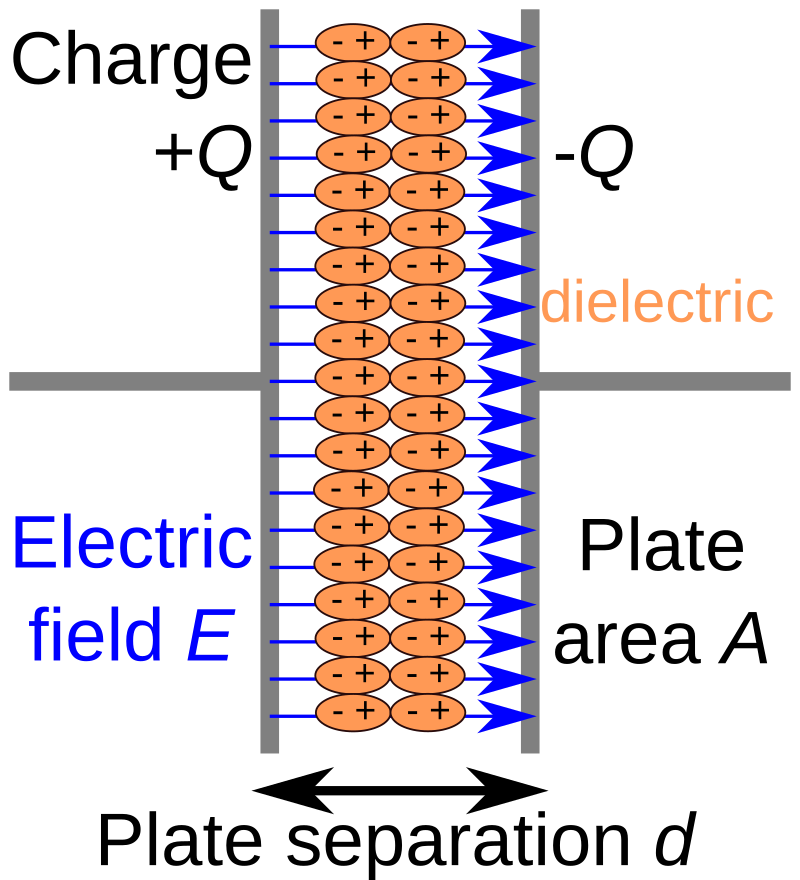
\includegraphics[width=0.35\textwidth]{figures/dielectrics.png}
    \caption{Schematic representation of a dielectric. The external electric field polarizes the material causing dipoles to point opposite to the electric field}
    \label{fig:dielectrics}
\end{figure}

\section{Superconductivity}
There are two types of superconductors. Conventional ones, and unconvential ones.
The standard theory of superconductivity, named BCS theory after Bardeen, Cooper, and Schrieffer, uses the same basic principles to explain superconductivity as more advanced models. These principles are also a key part of describing ferroelectric superconducting heterostructures. In BCS theory, it is shown that under the right conditions, two electrons can form bound pairs at an energy below the Fermi level.

\subsection{Standard BCS Theory}
In standard BCS theory, the conditions for forming bound pairs of electrons are as follows. The two electrons are assumed to be in a free electrons, added to a Fermi sea at a temperature of 0K. These electrons interact with eachother, through both an electric repulsion from a screened Coulomb interaction, and another iteraction mediated by phonons. The phonon-mediated interaction here is key. Scattering of one of the electrons from a momentum \textbf{k} to a momentum \textbf{k'}. This creates a phonon of momentum \textbf{k} - \textbf{k'} = \textbf{q}, that is carried through the atom core oins in the material. This process is shown schematically in figure \ref{fig:electron_phonon} .

\begin{figure}[h]
    \centering
    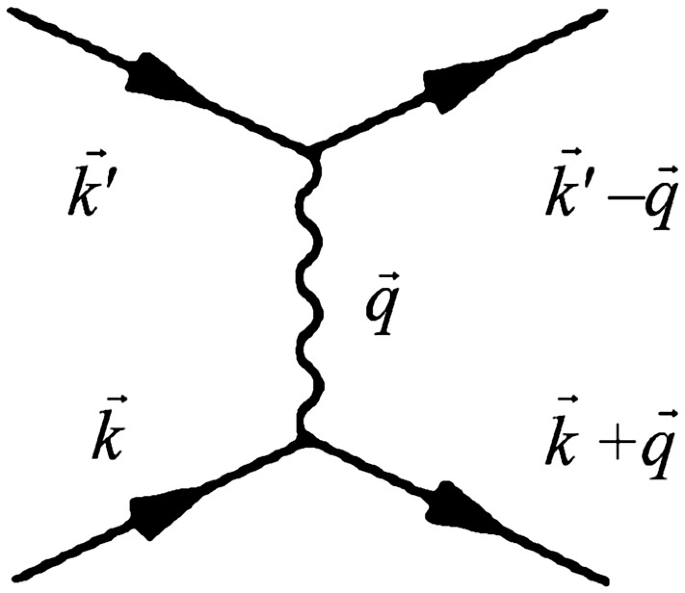
\includegraphics[width=0.25\textwidth]{figures/electron_phonon.png}
    \caption{Schematic representation of electron-electron interaction mediated by a phonon with momentum \textbf{q} = \textbf{k-k'}}
    \label{fig:electron_phonon}
\end{figure}

It is shown by de Gennes \cite{Gennes} using the so-called "jellium model" that this gives rise to an effective attractive interaction between the two electrons given by 
\begin{equation}
    V(\textbf{q}, \omega) = \frac{4 \pi (e^+)^2}{q^2 + {k_s}^2} \left( 1 + \frac{\omega_\textbf{q}^2}{\omega^2 - \omega_\textbf{q}^2} \right)
\end{equation}
Where $\frac{1}{k_s}$ is the screening length, also known as the screening constant $\kappa$, $\omega_\mathbf{q}$ is the characteristic frequency of the phonon, and $\omega$ is the characteristic frequency of the electrons, defined by $\hbar \omega = \xi_\textbf{k'} = \xi_\textbf{k}$, with $\xi_\textbf{k}$ being the energy of the electron with momentum \textbf{k}.

\section{Screening} 
In conductors, electric fields behave differently to in a vacuum. The presence of positively charged ions and negatively charged electrons cause electric potentials to drop exponentially with distance. Using the Thomas-Fermi approximation \cite{Ashcroft}, we find a dielectric function,
\begin{equation}
    \epsilon(r) = \epsilon_0 e^{\kappa r}
\end{equation}
Where $\kappa$ is the so-called screening constant. Or in other words, all electric potentials are multiplied by an $e^{\kappa r}$ term.
